
% prime.tex — حواف العدّ والحساب — Prime — النسخة المعدلة للرفع
% Compiler: XeLaTeX
\documentclass[12pt,a4paper]{article}
\usepackage{amsmath,amssymb}
\usepackage{graphicx}
\usepackage{booktabs}
\usepackage{array}
\usepackage[margin=2.2cm]{geometry}
\usepackage{xcolor}
\usepackage{float}
\usepackage{fontspec}
\usepackage{polyglossia}
\usepackage{hyperref}
\setmainlanguage[numerals=maghrib]{arabic}
\setotherlanguage{english}
\setmainfont{Amiri}
\usepackage{fancyhdr}
\pagestyle{fancy}
\fancyhf{}
\fancyhead[L]{\small \textenglish{Edges of Counting and Computation — Prime}}
\fancyhead[R]{\small \textenglish{M. N. Al-Jabri (2026)}}
\fancyfoot[L]{\scriptsize \textenglish{Abdulla M. N. Al-Jabri | ORCID: 0009-0003-3319-3822}}
\fancyfoot[C]{\scriptsize \textenglish{Zenodo DOI: to be assigned}}
\fancyfoot[R]{\small \thepage}
\renewcommand{\headrulewidth}{0.4pt}
\renewcommand{\footrulewidth}{0.4pt}
\fancypagestyle{firstpage}{
  \fancyhf{}
  \fancyfoot[C]{عبدالله محمد ناصر الجبري — حواف العدّ والحساب — Prime — \thepage}
  \renewcommand{\headrulewidth}{0pt}
  \renewcommand{\footrulewidth}{0pt}
}
\title{\textbf{حواف العدّ والحساب — \textenglish{Prime}}}
\author{عبدالله محمد ناصر الجبري \\
صنعاء، اليمن \\
\textenglish{ORCID: 0009-0003-3319-3822} \\
\textenglish{Email: jabri62018@gmail.com} \\
\textenglish{Portal: \url{https://jabri-com.vercel.app}} \\
\textenglish{Zenodo DOI: to be assigned on deposit}}
\date{21 نوفمبر 2026م}
\begin{document}
\maketitle
\thispagestyle{firstpage}

% --- Reproducibility — first page, DOI/Zenodo ---
\begin{center}
\fbox{\parbox{0.92\textwidth}{
\textbf{إعادة الإنتاج والمواد الحسابية (\textenglish{Reproducibility and Computational Materials})}\\[2mm]
السكربتات الحسابية، وإجراءات معالجة البيانات، والمواد الداعمة المستخدمة لتوليد النتائج المعروضة متاحة في:\\[1mm]
\textbf{مستودع \textenglish{GitHub}:} [\textenglish{Repository Link}]\\[1mm]
\textbf{الإصدار المؤرشف:} [\textenglish{Release Link}]\\[1mm]
الإصدار المؤرشف هو الإصدار المستخدم في هذه الدراسة، ويوفر المواد اللازمة لفحص الحسابات المعروضة وإعادة إنتاجها. وتقتصر مواد إعادة الإنتاج على النتائج المعروضة بالفعل في هذه الورقة؛ ولا يُوعد بإعادة إنتاج نتائج اختبارات لم تُغلق بعد، ومنها \textenglish{M1-E}، إلا بعد إغلاقها وتثبيت إصدارها.
}}
\end{center}
\vspace{0.3cm}

\begin{center}
\textbf{نعدّ الأوليات، نحسب حوافها، ونعرض ما أظهرته المقارنات بين نطاقاتها.}
\end{center}
\begin{center}
\small عبدالله محمد ناصر الجبري \quad $\cdot$ \quad صنعاء، اليمن \quad $\cdot$ \quad \textenglish{ORCID: 0009-0003-3319-3822} \quad $\cdot$ \quad \textenglish{Email: jabri62018@gmail.com}
\end{center}
\vspace{0.5cm}

% ==========================================
\section{الملخص (\textenglish{Abstract})}
تعرض هذه الدراسة نتائج المسح الحسابي وتحليل الفجوات الأولية ضمن النطاق المحدد، مع توثيق منهج استخراج البيانات والقياسات والاختبارات المستخدمة. ونترك تقييم النتائج ودلالاتها وموقع هذا العمل للقارئ والمحكّمين.

تستقصي الورقة السلوك الإحصائي للفجوات بين الأعداد الأولية المتتالية $g_n = p_{n+1} - p_n$ وصولاً إلى الحد الحسابي $N = 10^9$ (مليار). نتبع دالة الانحراف $D_1(x) = \pi(x) - \mathrm{Li}(x)$، وكثافة الأوليات $\rho_k$، وتوزيع تكرارات الفجوات عبر ثلاثة نطاقات حسابية مقارنة ($B, C, D$)، وهي نطاقات من السلسلة الحسابية نفسها، وليست تشغيلات مستقلة.

تُظهر النتائج أن $D_1(x)$ كانت سالبة في جميع نقاط القياس المُوثّقة في الجدول التراكمي، وتناقصًا في كثافة الأوليات عبر النوافذ المتتابعة التي جرى قياسها، بما يتسق مع مبرهنة الأعداد الأولية. كما تُظهر النتائج اختلافًا في ترتيب تكرار الفجوات بين النطاقات العددية التي تمت دراستها، بما يشير إلى أن هذا الترتيب ليس ثابتًا عبر النطاقات المقارنة. وتستكشف الدراسة العلاقة بين تغير كثافة الأوليات وتوزيع الفجوات، دون افتراض وجود علاقة سببية مسبقة.

% ==========================================
\section{المقدمة والمشكلة والفرضية}
تُعدّ الأعداد الأولية اللبنات الأساسية لنظرية الأعداد، وعلى الرغم من حتمية تعريفها، فإن توزيعها الموضعي يظهر سلوكًا شبه عشوائي يثير تساؤلات حول وجود ارتباطات بين الفجوات المتتالية.

\begin{itemize}
    \item \textbf{المشكلة البحثية:} هل تمتلك الفجوات بين الأعداد الأولية المتتالية «ذاكرة» إحصائية أو بنية انتقال متكررة؟ وتُستخدم كلمة «ذاكرة» هنا بمعنى إحصائي تشغيلي، أي وجود ارتباط قابل للقياس بين فجوة وأخرى لاحقة، وليس بمعنى آلية في الأعداد الأولية.
    \item \textbf{الفرضية الصفرية (قبل الحساب):} افترضنا مبدئيًا أن أحجام الحواف تتصرف كمتغيرات مستقلة إحصائيًا، وأن الترتيب النسبي لتكرار الحواف الأكثر شيوعًا (مثل $2, 4, 6$) يظل مستقرًا عبر النطاقات العددية المقارنة.
    \item \textbf{منهجية الاختبار:} فحص ما إذا كانت فئة حجم الحافة الحالية $g_n$ تحمل معلومة إحصائية تؤثر في الحافة اللاحقة $g_{n+1}$، ومقارنة ترتيب التكرار عبر ثلاثة نطاقات حسابية مقارنة ($B$ و $C$ و $D$).
\end{itemize}

\noindent \textbf{ما يقدمه هذا العمل:} استخراج سلسلة الفجوات حتى مليار، قياس الانحراف عن $\mathrm{Li}(x)$، متابعة تغير كثافة الأوليات، تحليل توزيع أحجام الفجوات، مقارنة ترتيب تكرارات الفجوات عبر النطاقات، اختبار الارتباط بين الفجوات المتتابعة، واختبار أكثر دقة لمعرفة ما إذا كانت القيمة الدقيقة للفجوة تضيف معلومات فوق تصنيفها.

% ==========================================
\section{الهوية الرسمية للبحث}
\begin{figure}[H]
\centering
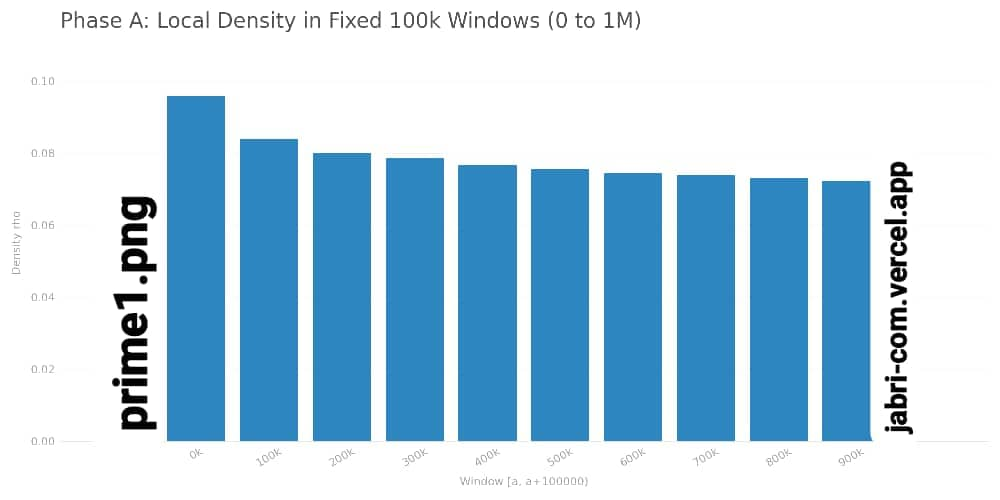
\includegraphics[width=0.92\textwidth]{prime1.png}
\caption{بطاقة الهوية الرسمية لمشروع البحث — \textenglish{Prime}}
\end{figure}
\begin{table}[H]
\centering
\begin{tabular}{ll}
\toprule
\textbf{العنصر} & \textbf{المعتمد} \\
\midrule
الاسم & عبدالله محمد ناصر الجبري \\
الاسم بالإنجليزية & \textenglish{Abdulla M. N. Al-Jabri} \\
العنوان & صنعاء، اليمن \\
\textenglish{ORCID} & \textenglish{0009-0003-3319-3822} \\
البريد الإلكتروني & \textenglish{jabri62018@gmail.com} \\
\textenglish{Zenodo DOI} & \textenglish{to be assigned on deposit} \\
اسم العمل & حواف العدّ والحساب \\
الرمز المرجعي & \textenglish{Prime} \\
التعريف الرياضي & $g_n = p_{n+1} - p_n$ \\
المنهج & استخراج الأوليات، حساب الحواف، والتحليل الإحصائي للنوافذ \\
السؤال البحثي & هل للفجوات ذاكرة؟ (بمعنى إحصائي تشغيلي) \\
التاريخ & 21 نوفمبر 2026م \\
\bottomrule
\end{tabular}
\caption{البيانات الوصفية والمرجعية للورقة البحثية}
\end{table}

% ==========================================
\section{التعريف والاشتقاق الرياضي}
\subsection{تعريف الحافة (\textenglish{Prime Gap})}
تُعرَّف الحافة رقم $n$ بأنها المسافة الحسابية (الفرق) بين عددين أوليين متتاليين:
\[
g_n = p_{n+1} - p_n, \quad \forall n \geq 1
\]
\subsection{خوارزمية استخراج الحواف}
\begin{enumerate}
    \item \textbf{الغربال:} تطبيق غربال إراتوستينس (\textenglish{Sieve of Eratosthenes}) لاستخراج كافة الأعداد الأولية حتى الحد $N = 10^9$، مع استبعاد العدد $1$ صراحةً من مجموعة الأوليات.
    \item \textbf{حساب الفروق:} طرح كل عدد أولي $p_n$ من العدد الأولي الذي يليه مباشرة $p_{n+1}$.
    \item \textbf{الحافة الابتدائية:} الحافة الأولى هي $g_1 = 3 - 2 = 1$، وهي الحالة الفردية الوحيدة؛ إذ إن كل عدد أولي $p_n > 2$ هو عدد فردي بالضرورة، والفرق بين أي عددين فرديين هو عدد زوجي حتمًا ($g_n \equiv 0 \pmod 2$ لكل $n \geq 2$).
\end{enumerate}
\subsection{مثال مصغر للتوضيح}
\begin{table}[H]
\centering
\begin{tabular}{cccc}
\toprule
\textbf{الرتبة ($n$)} & \textbf{الأولي الحالي ($p_n$)} & \textbf{الأولي التالي ($p_{n+1}$)} & \textbf{الحافة ($g_n$)} \\
\midrule
1 & 2 & 3 & 1 \\
2 & 3 & 5 & 2 \\
3 & 5 & 7 & 2 \\
4 & 7 & 11 & 4 \\
5 & 11 & 13 & 2 \\
\bottomrule
\end{tabular}
\caption{نموذج تطبيقي لحساب الحواف الخمس الأولى}
\end{table}
\subsection{دوال العدّ والانحراف والكثافة}
\begin{itemize}
    \item $\pi(x)$: دالة عدّ الأوليات الفعلية التي تقل عن أو تساوي $x$.
    \item $\mathrm{Li}(x) = \mathrm{Ei}(\ln x) - \mathrm{Ei}(\ln 2) = \int_2^x \frac{dt}{\ln t}$: التكامل اللوغاريتمي.
    \item $x / \ln x$: التقريب الكلاسيكي لمبرهنة الأعداد الأولية.
    \item $D_1(x) = \pi(x) - \mathrm{Li}(x)$: الانحراف الأول.
    \item $D_2(x) = \pi(x) - x/\ln x$: الانحراف الثاني.
    \item $R(x) = |D_1(x)| / \pi(x)$: الخطأ النسبي للانحراف الأول.
    \item $\rho_k = (\pi(b_k) - \pi(a_k)) / 10^8$: كثافة الأوليات داخل النافذة القياسية $k$ ذات العرض $10^8$.
    \item $\bar{g}_k = 1 / \rho_k$: التباعد المتوسط المقدّر من الكثافة، وليس المتوسط المحسوب مباشرة من الفجوات، وهو $\bar{g}_k^{\,\mathrm{actual}} = (1/m_k)\sum_{j=1}^{m_k} g_j$.
    \item $\Delta D_1$: مقدار التغيّر في قيمة $D_1$ مقارنة بنقطة القياس السابقة.
\end{itemize}
\subsection{قاعدة العدّ في النطاق \textenglish{D} وتصنيف فئات \textenglish{M1}}
\textbf{شرط الانتماء للنطاق \textenglish{D}:} تُقبل الحافة $g_n = p_{n+1} - p_n$ ضمن إحصاءات النطاق $D$ فقط إذا تحقق: $p_{n+1} > 10^8$ ($100\text{M}$).
\noindent \textbf{فئات التصنيف الحجمي (\textenglish{M1}):}
\begin{itemize}
    \item \textbf{صغيرة (\textenglish{Small}):} $g \leq 6$ (وتشمل القيم $1, 2, 4, 6$).
    \item \textbf{متوسطة (\textenglish{Medium}):} $8 \leq g \leq 14$ (وتشمل القيم $8, 10, 12, 14$).
    \item \textbf{كبيرة (\textenglish{Large}):} $g \geq 16$.
\end{itemize}
\noindent \textbf{الدقة الرياضية:} تحديد الفئة المتوسطة بالمدى $[8, 14]$ تحديد شامل؛ لأن الحافة الفردية الوحيدة ($g_1 = 1$) محتواة داخل الفئة الصغيرة، وجميع الحواف اللاحقة أعداد زوجية، مما ينفي وجود حافة قيمتها $7$ أو $15$.

% ==========================================
\section{التصميم التجريبي والنتائج الحسابية}
تم تقسيم العرض إلى ثلاث نطاقات حسابية مقارنة ($B, C, D$) لرصد المؤشرات الثلاثة: الانحراف $D_1$، الكثافة $\rho_k$، وتوزيع تكرار الحواف. هذه النطاقات مقاطع من السلسلة الحسابية نفسها، وتُستخدم للمقارنة، وليست تشغيلات مستقلة إحصائيًا.

\subsection{نتائج النطاق \textenglish{B}}
\begin{figure}[H]\centering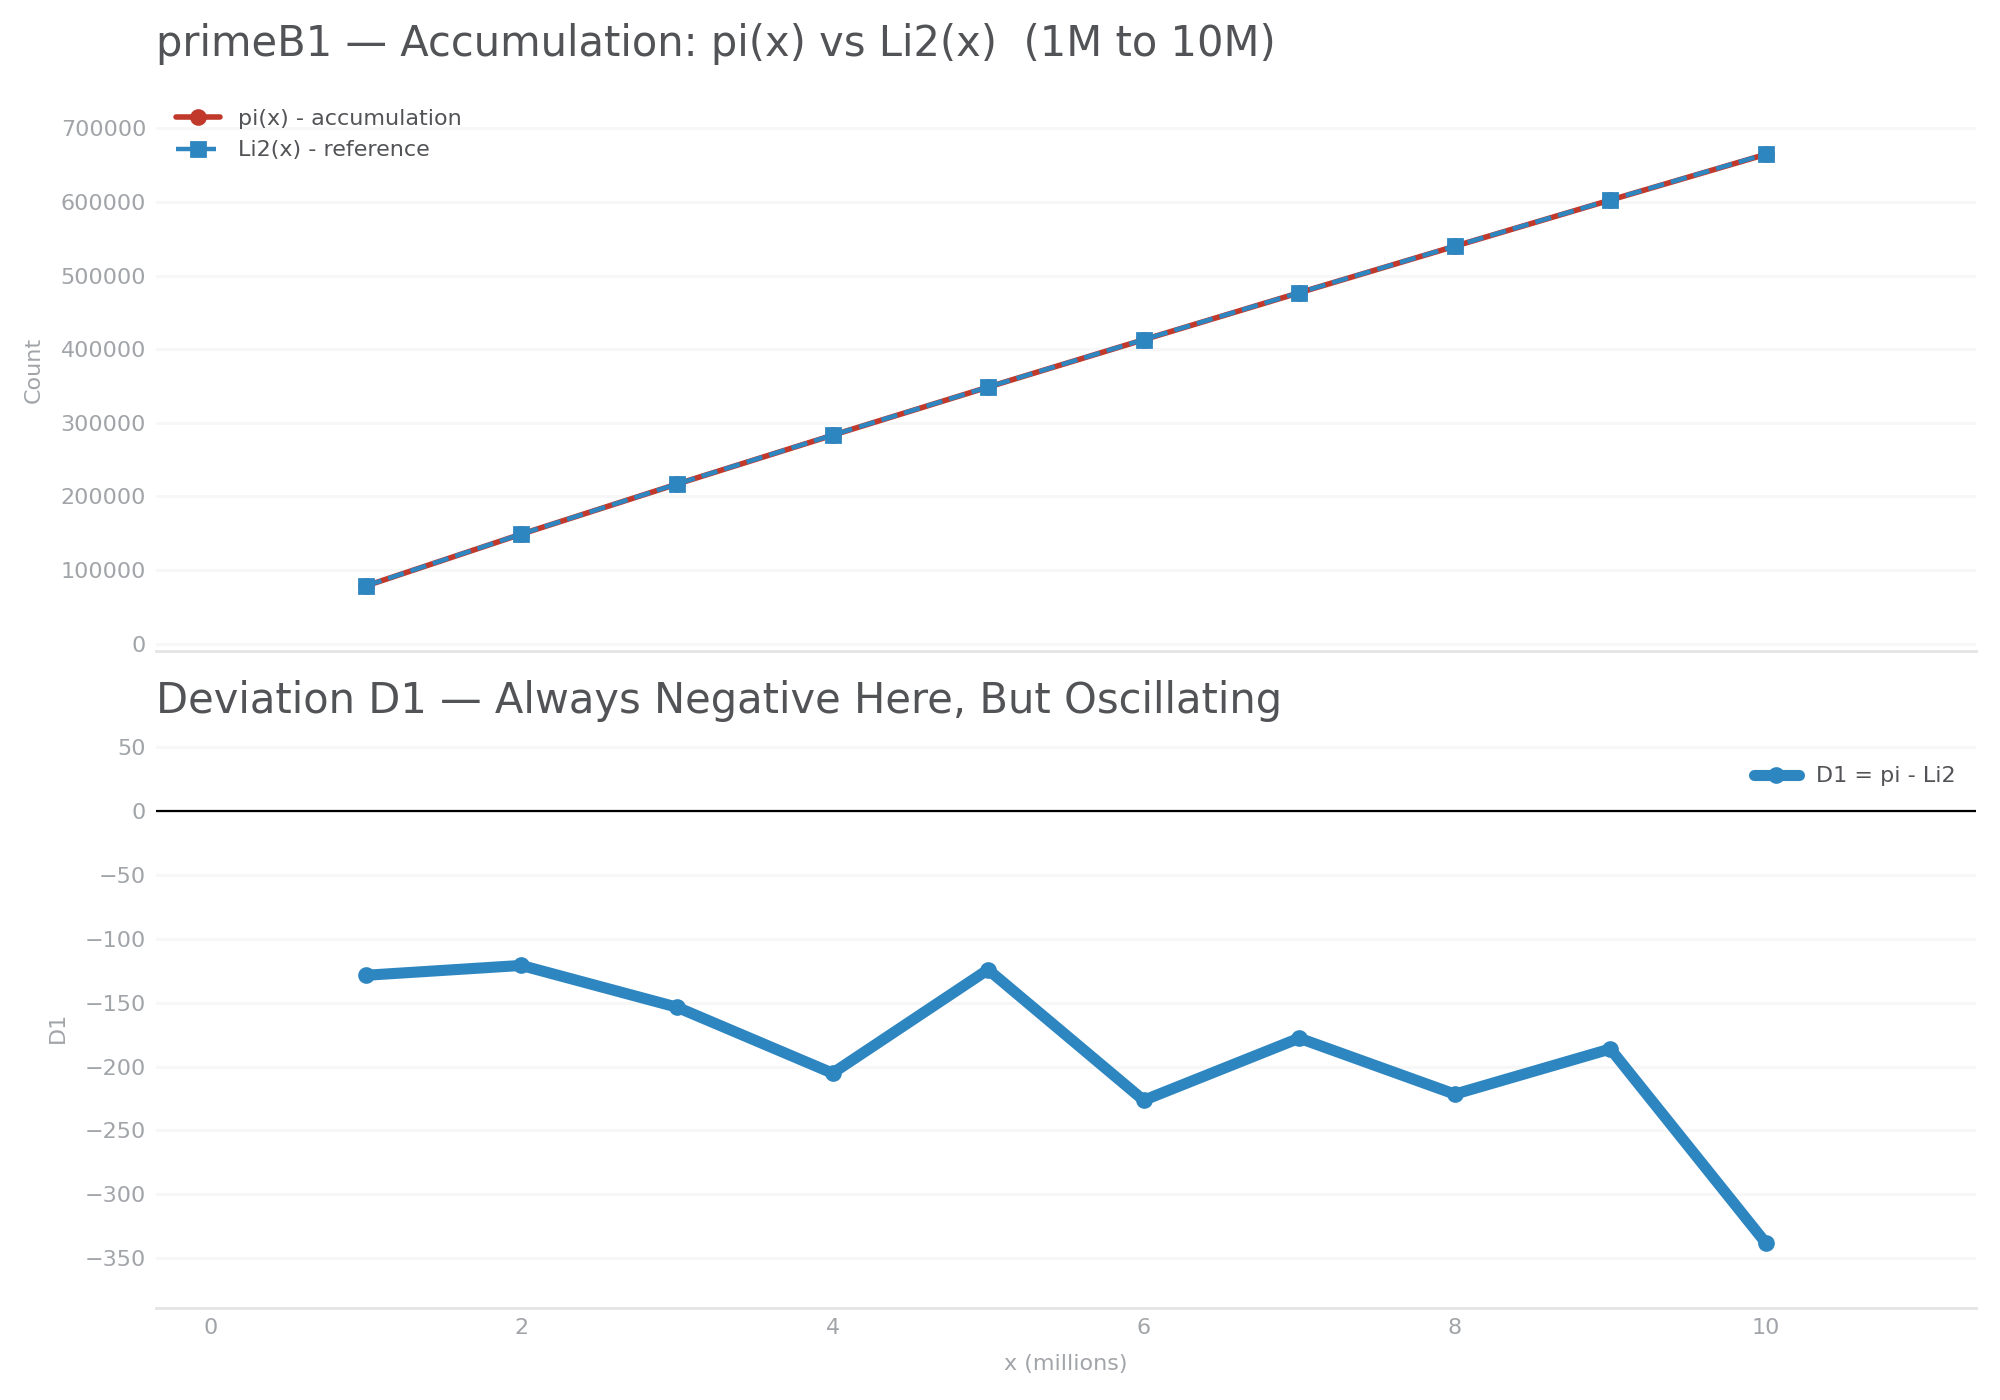
\includegraphics[width=0.85\textwidth]{primeB1.png}\caption{النطاق \textenglish{B}: تطور دالة الانحراف $D_1(x)$}\end{figure}
\begin{figure}[H]\centering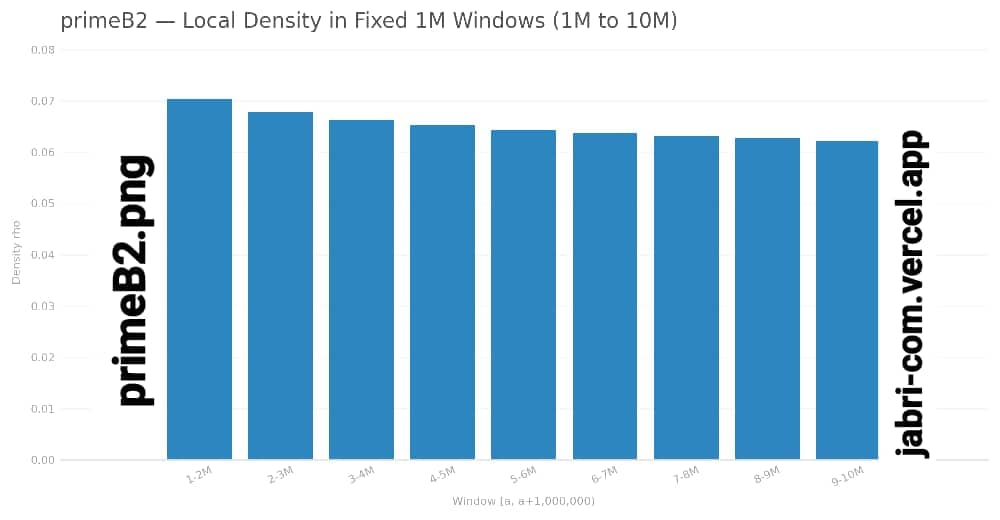
\includegraphics[width=0.85\textwidth]{primeB2.png}\caption{النطاق \textenglish{B}: منحنى كثافة الأوليات $\rho_k$}\end{figure}
\begin{figure}[H]\centering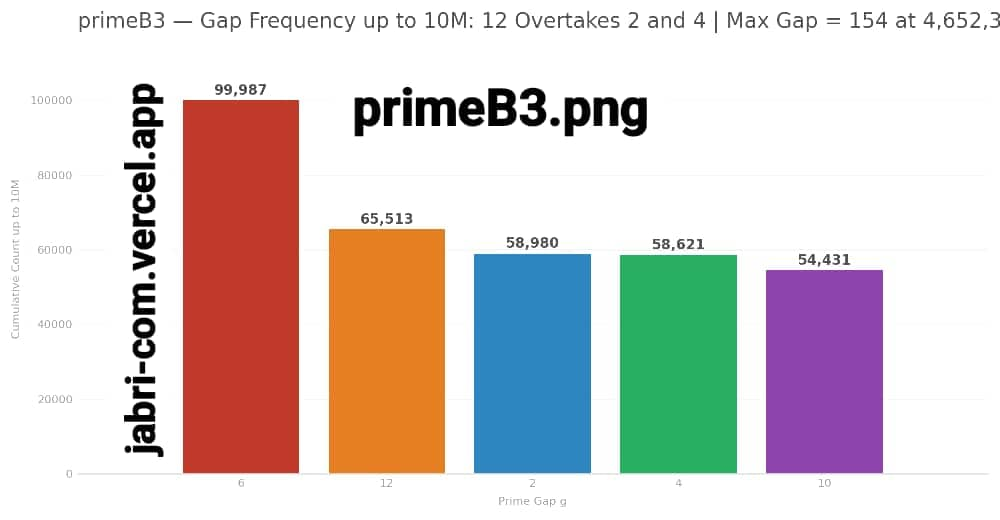
\includegraphics[width=0.85\textwidth]{primeB3.png}\caption{النطاق \textenglish{B}: توزيع تكرارات الحواف}\end{figure}

\subsection{نتائج النطاق \textenglish{C}}
\begin{figure}[H]\centering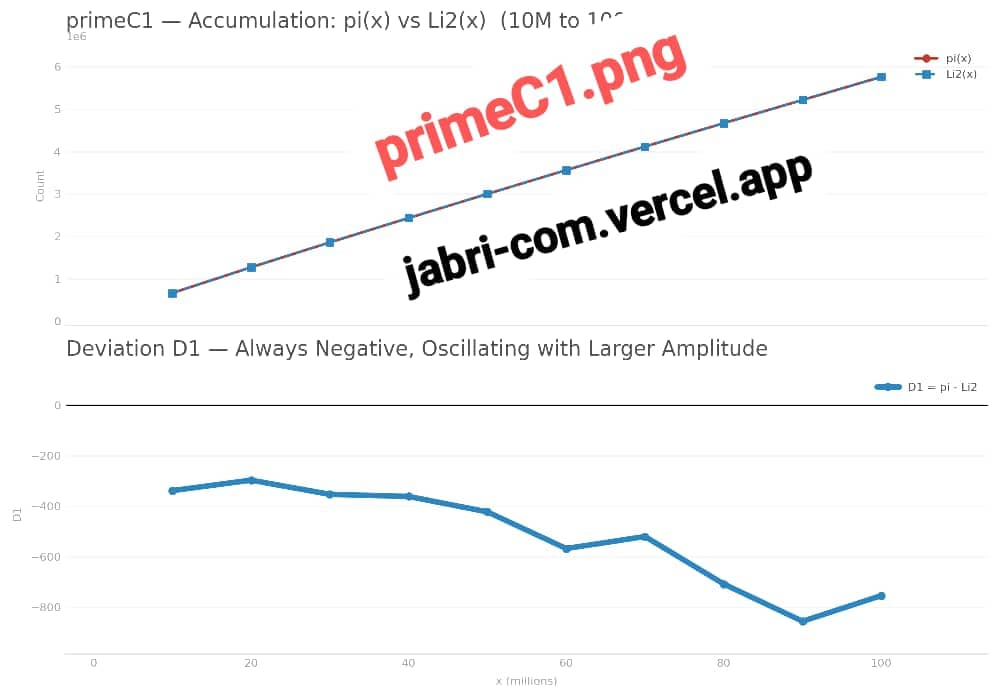
\includegraphics[width=0.85\textwidth]{primeC1.png}\caption{النطاق \textenglish{C}: تطور دالة الانحراف $D_1(x)$}\end{figure}
\begin{figure}[H]\centering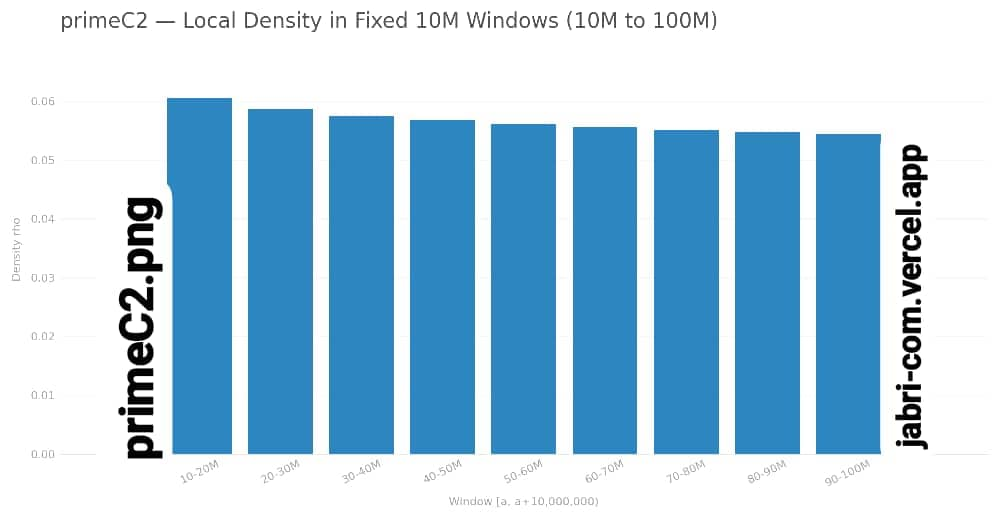
\includegraphics[width=0.85\textwidth]{primeC2.png}\caption{النطاق \textenglish{C}: منحنى كثافة الأوليات $\rho_k$}\end{figure}
\begin{figure}[H]\centering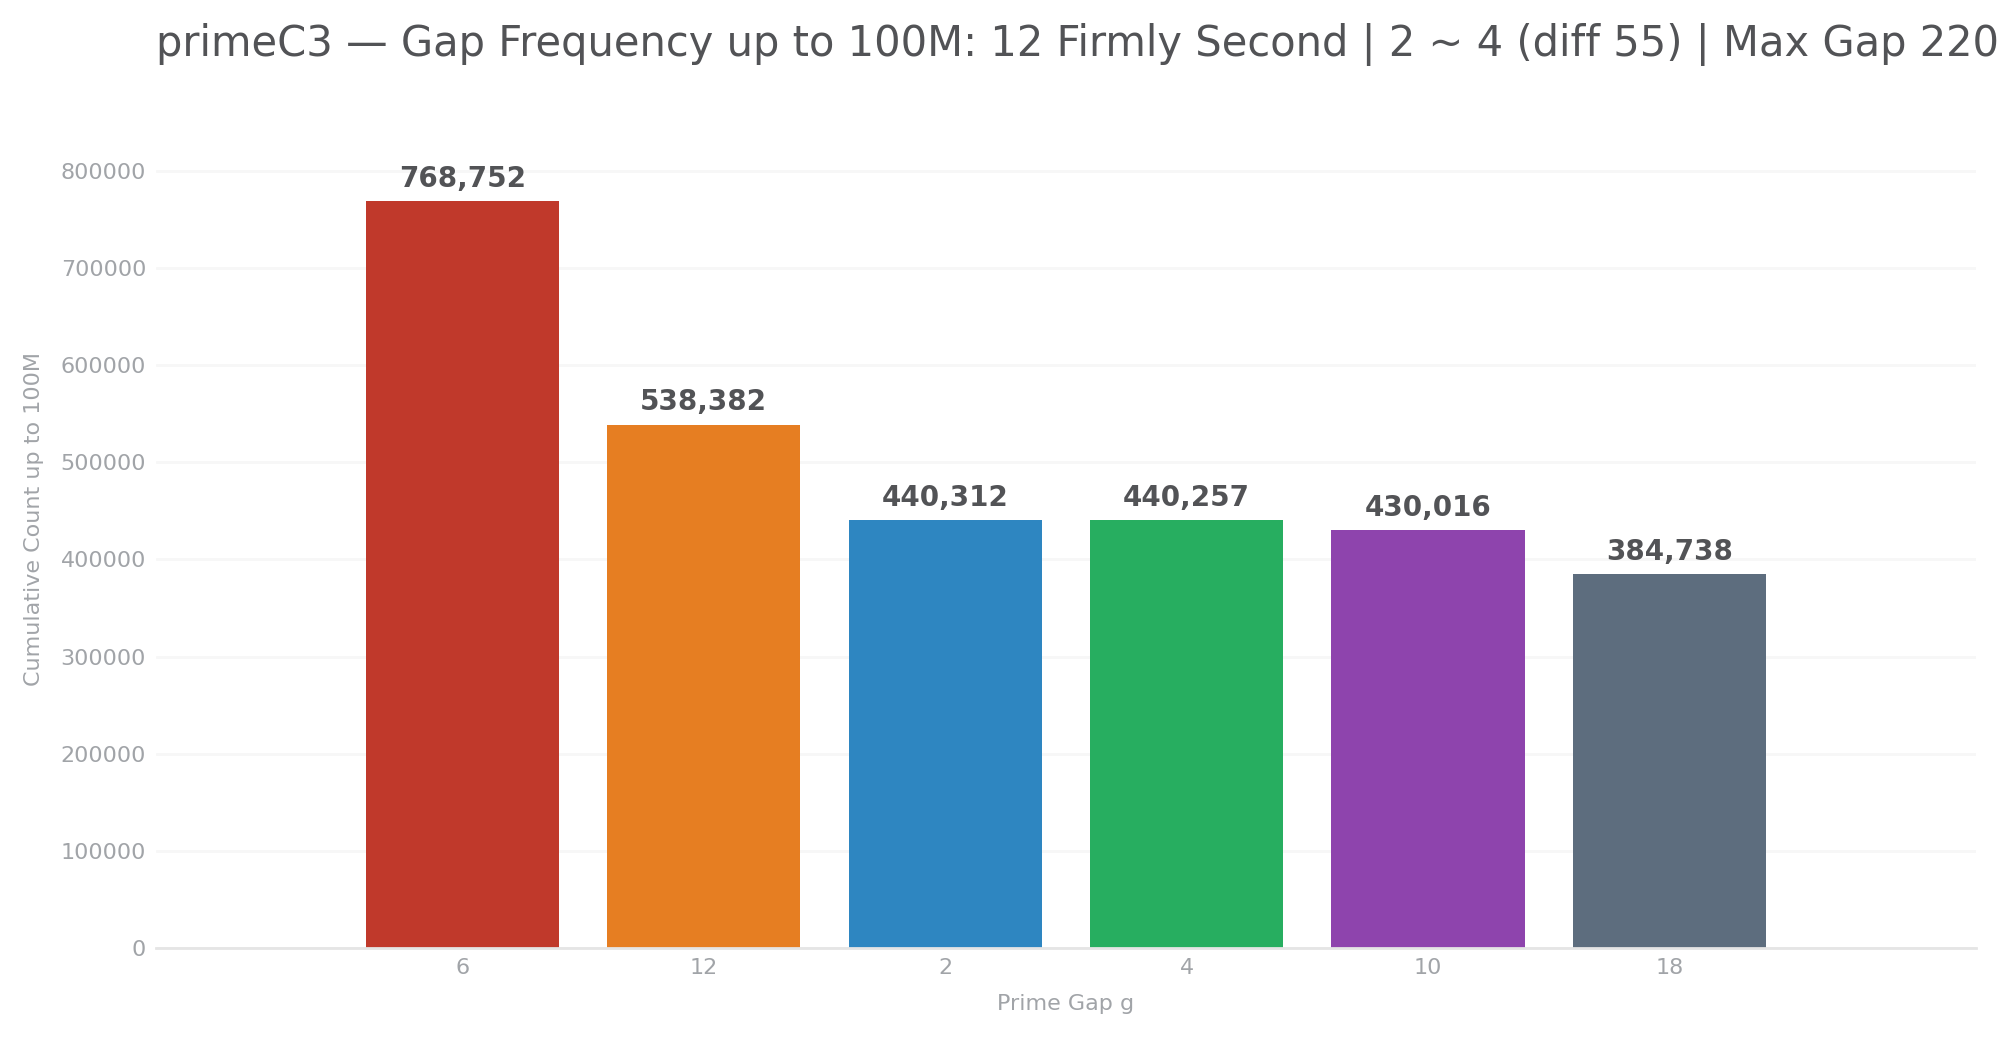
\includegraphics[width=0.85\textwidth]{primeC3.png}\caption{النطاق \textenglish{C}: توزيع تكرارات الحواف}\end{figure}

\subsection{نتائج النطاق \textenglish{D} (ما فوق $100\text{M}$ حتى $10^9$)}
\begin{figure}[H]\centering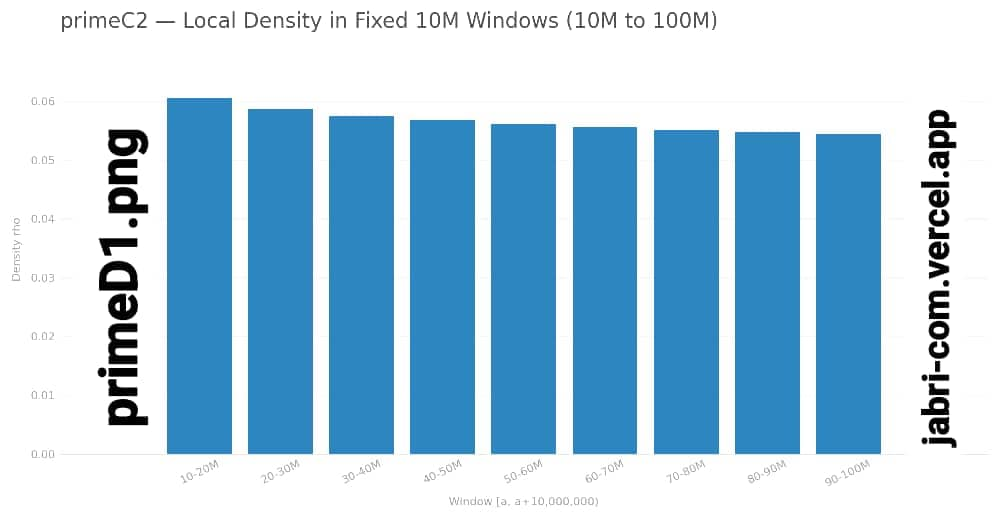
\includegraphics[width=0.85\textwidth]{primeD1.png}\caption{النطاق \textenglish{D}: سلوك دالة الانحراف $D_1(x)$ فوق $10^8$}\end{figure}
\begin{figure}[H]\centering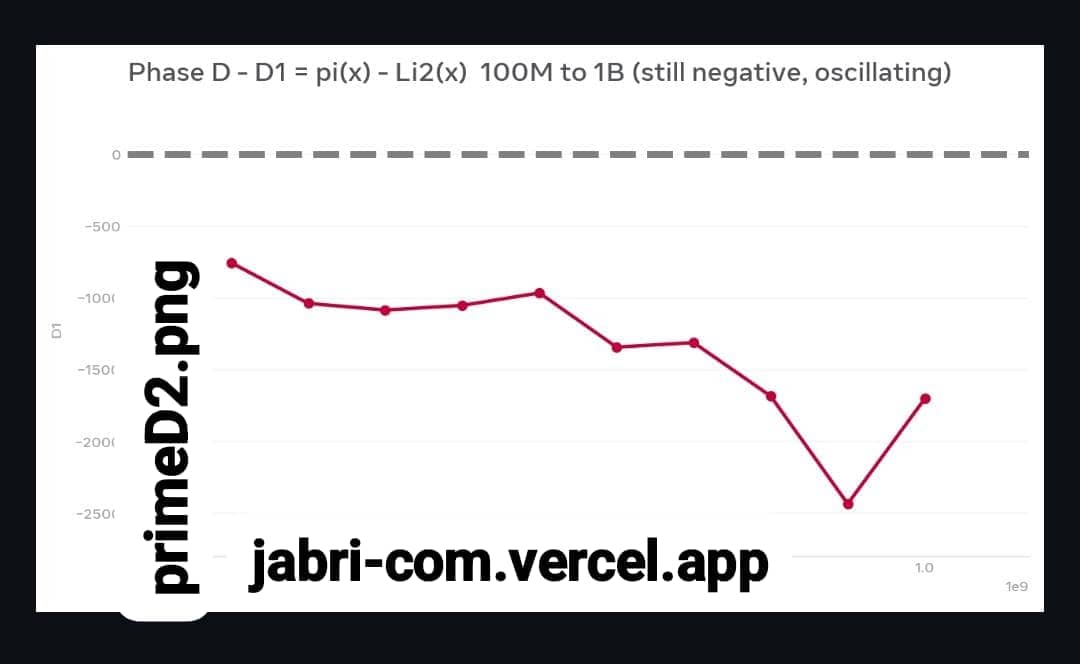
\includegraphics[width=0.85\textwidth]{primeD2.png}\caption{النطاق \textenglish{D}: تراجع الكثافة $\rho_k$ وارتفاع متوسط الحافة $\bar{g}_k$}\end{figure}
\begin{figure}[H]\centering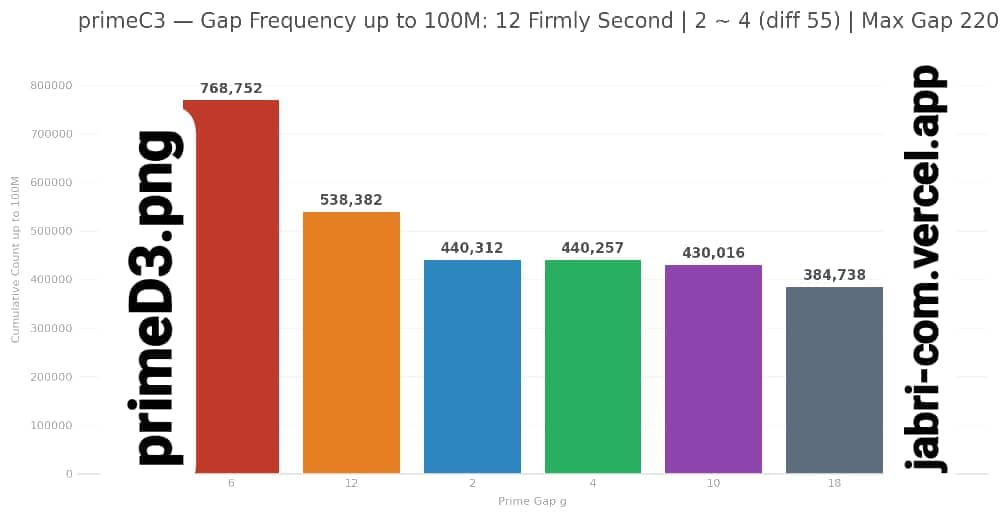
\includegraphics[width=0.85\textwidth]{primeD3.png}\caption{النطاق \textenglish{D}: اختلاف ترتيب تكرار الحواف}\end{figure}

\begin{table}[H]
\centering\small
\begin{tabular}{rrrrrrr}
\toprule
$x$ & $\pi(x)$ & $\mathrm{Li}(x)$ & $D_1$ & $\Delta D_1$ & $D_2$ & $R(x)$ \\
\midrule
$100{,}000{,}000$ & $5{,}761{,}455$ & $5{,}762{,}208.3$ & $-753.3$ & $-753.3$ & $332{,}774.0$ & $0.000131$ \\
$200{,}000{,}000$ & $11{,}078{,}937$ & $11{,}079{,}973.8$ & $-1{,}036.8$ & $-283.5$ & $615{,}308.2$ & $0.000094$ \\
$300{,}000{,}000$ & $16{,}252{,}325$ & $16{,}253{,}408.1$ & $-1{,}083.1$ & $-46.3$ & $882{,}915.9$ & $0.000067$ \\
$400{,}000{,}000$ & $21{,}336{,}326$ & $21{,}337{,}377.0$ & $-1{,}051.0$ & $+32.1$ & $1{,}141{,}420.0$ & $0.000049$ \\
$500{,}000{,}000$ & $26{,}355{,}867$ & $26{,}356{,}831.1$ & $-964.1$ & $+86.9$ & $1{,}393{,}458.7$ & $0.000037$ \\
$600{,}000{,}000$ & $31{,}324{,}703$ & $31{,}326{,}044.207$ & $-1{,}341.207$ & $-377.103$ & $1{,}640{,}014.082$ & $0.000042816$ \\
$700{,}000{,}000$ & $36{,}252{,}931$ & $36{,}254{,}240.999$ & $-1{,}309.999$ & $+31.208$ & $1{,}882{,}917.694$ & $0.000036135$ \\
$800{,}000{,}000$ & $41{,}146{,}179$ & $41{,}147{,}861.2$ & $-1{,}682.2$ & $-372.2$ & $2{,}122{,}021.5$ & $0.000041$ \\
$900{,}000{,}000$ & $46{,}009{,}215$ & $46{,}011{,}647.6$ & $-2{,}432.6$ & $-750.4$ & $2{,}357{,}836.0$ & $0.000053$ \\
$1{,}000{,}000{,}000$ & $50{,}847{,}534$ & $50{,}849{,}233.912$ & $-1{,}699.912$ & $+732.688$ & $2{,}592{,}591.566$ & $0.000033432$ \\
\bottomrule
\end{tabular}
\caption{الجدول التراكمي — كل 100 مليون. القيم المعروضة هي نقاط قياس، وسالبية $D_1$ مرصودة في هذه النقاط.}
\end{table}

\begin{table}[H]
\centering
\begin{tabular}{rrrr}
\toprule
النافذة & أوليات النافذة & $\rho_k$ & $\bar{g}_k$ \\
\midrule
100M -- 200M & $5{,}317{,}482$ & $0.053175$ & $18.806$ \\
200M -- 300M & $5{,}173{,}388$ & $0.051734$ & $19.330$ \\
300M -- 400M & $5{,}084{,}001$ & $0.050840$ & $19.670$ \\
400M -- 500M & $5{,}019{,}541$ & $0.050195$ & $19.922$ \\
500M -- 600M & $4{,}968{,}836$ & $0.049688$ & $20.125$ \\
600M -- 700M & $4{,}928{,}228$ & $0.049282$ & $20.291$ \\
700M -- 800M & $4{,}893{,}248$ & $0.048932$ & $20.436$ \\
800M -- 900M & $4{,}863{,}036$ & $0.048630$ & $20.563$ \\
900M -- 1B & $4{,}838{,}319$ & $0.048383$ & $20.668$ \\
\bottomrule
\end{tabular}
\caption{الكثافة في نوافذ D التسع}
\end{table}

\begin{table}[H]
\centering
\begin{tabular}{rrr}
\toprule
المرتبة & الفجوة & التكرار في D \\
\midrule
1 & 6 & $5{,}321{,}039$ \\
2 & 12 & $3{,}930{,}575$ \\
3 & 10 & $3{,}054{,}751$ \\
4 & 4 & $2{,}984{,}422$ \\
5 & 2 & $2{,}984{,}194$ \\
6 & 18 & $2{,}966{,}294$ \\
7 & 8 & $2{,}360{,}929$ \\
8 & 14 & $2{,}171{,}364$ \\
9 & 24 & $2{,}109{,}926$ \\
10 & 30 & $1{,}955{,}144$ \\
11 & 16 & $1{,}630{,}293$ \\
12 & 20 & $1{,}621{,}121$ \\
13 & 22 & $1{,}393{,}734$ \\
14 & 28 & $1{,}089{,}676$ \\
15 & 36 & $1{,}057{,}496$ \\
\bottomrule
\end{tabular}
\caption{تكرار الحواف الخمس عشرة الأولى في D — الإجمالي 45,086,079}
\end{table}

% ==========================================
\section{اختبار الذاكرة الإضافية للقيمة الدقيقة للفجوة (\textenglish{M1-E})}
يختبر نموذج \textenglish{M1} العلاقة $P(S_{n+1}\mid S_n)$، بينما يختبر \textenglish{M1-E} إمكانية تحسين التنبؤ باستخدام القيمة الدقيقة:
\[
P(S_{n+1}\mid g_n).
\]
والسؤال هو: هل يضيف $g_n$ معلومات تنبؤية تتجاوز $S_n$ عند توقع $S_{n+1}$؟
\paragraph{بروتوكول الاختبار (مجمّد، قيد التنفيذ).}
\begin{enumerate}
    \item تقسيم زمني متتابع $50\%/50\%$: النصف الأول تدريب، والثاني اختبار. لا تُخلط الانتقالات عشوائيًا.
    \item تمثيل قيم الفجوات الدقيقة حتى $30$، واستخدام فئات لوغاريتمية ثابتة للفجوات الأكبر.
    \item حد دمج مقداره $200$، ونظام دمج تصاعدي ثابت، مع تنعيم لابلاس $\alpha=1$. تفاصيل الدمج: تُدمج الفئات النادرة تصاعديًا من الأكبر إلى الأصغر حتى يصل عدد كل فئة مدمجة إلى الحد $200$ على الأقل في التدريب؛ وعند التعادل في التردد يُكسر التعادل باختيار القيمة الأصغر أولًا، وفق البذرة المحددة أدناه. هذا وصف لإعداد اختباري، وليس ضمانًا إحصائيًا.
    \item \textenglish{Block Bootstrap} بطول كتلة $100$ (إعداد اختباري ثابت)، وعدد تكرارات $B=2000$. الكتل المعاد أخذها نفسها لكلا النموذجين في كل تكرار (مقارنة مقترنة).
    \item تقييم التحسن باستخدام \textenglish{Log-Loss}، مع تقييم معامل \textenglish{Pearson} بصورة مستقلة وعدم دمج الحكمين.
    \item عدم تغيير البروتوكول بعد الاطلاع على النتائج.
\end{enumerate}
\paragraph{تعريفات التنفيذ.}
\begin{enumerate}
    \item \textbf{بيرسون، محدد:} معامل بيرسون المقيّم هو $r_1$ بين رمزي الفئتين المتتاليتين $S_n$ و $S_{n+1}$، مع ترميز الفئات: صغيرة $=1$، متوسطة $=2$، كبيرة $=3$. هذا الترميز يفرض ترتيبًا عدديًا على الفئات، لذا يُفسّر $r_1$ بوصفه ارتباطًا خطيًا رتبيًا على هذا الترميز تحديدًا، وليس مقياسًا عامًا لجميع أشكال الاعتماد.
    \item \textbf{البذرة:} \textenglish{SEED = 20261120} لإعادة الإنتاج للجزء العشوائي (Bootstrap وكسر التعادل). التقسيم الزمني حتمي. البذرة وحدها لا تثبت صحة النتيجة.
\end{enumerate}
\paragraph{حالة الاختبار.}
بروتوكول \textenglish{M1-E} محدد ومجمّد، إلا أن تنفيذه ونتيجته النهائية على بيانات الفجوات الأولية الفعلية ما زالا قيد التنفيذ. لذلك لا تُعرض أي نتيجة محاكاة بوصفها نتيجة محسوبة من السلسلة الأصلية، ولا تُصاغ نتيجة مسبقة.

\subsection{اختبار ترتيب الفئات والتحكم بالخلط العشوائي}
على سلسلة الفئات المرتبة، بلغ معامل الارتباط من الرتبة الأولى، على الترميز أعلاه:
\[
r_1=-0.03006.
\]
وهي قيمة ارتباط خطي سالب ضعيف. ولتمييز أثر الترتيب عن أثر توزيع الفئات الهامشي، يمكن إجراء اختبار تحكم بالخلط العشوائي، بحيث يُعاد ترتيب السلسلة مع المحافظة على التكرارات الأصلية. ولا يُفسر الارتباط السالب بمفرده بوصفه إثباتًا لآلية سببية محددة، كما لا يُعد غياب ارتباط خطي قوي دليلًا على غياب جميع أنواع الاعتماد.

% ==========================================
\section{المناقشة وصياغة الرصد التجريبي}
\subsection{تفسير النتائج}
\begin{enumerate}
\item \textbf{إشارة الانحراف في نقاط القياس:} كانت $D_1$ سالبة في جميع نقاط القياس الموثقة حتى $10^9$.
\item \textbf{تناقص الكثافة عبر النوافذ المقيسة:} انخفضت الكثافة $\rho_k$ عبر النوافذ المتتابعة، وهو ما يتسق مع التقريب $\rho(x) \sim 1/\ln x$.
\item \textbf{اختلاف ترتيب التكرار في النطاق \textenglish{D}:} أظهرت المقارنة اختلافًا في ترتيب تكرار الحواف مقارنة بالنطاقات الأدنى. هذا يُسجَّل كرصد للمقارنة، دون افتراض آلية.
\end{enumerate}
\subsection{الصياغة الرسمية للرصد التجريبي (\textenglish{Empirical Observation})}
\begin{quote}
\textbf{رصد تجريبي:} ضمن النطاق الحسابي حتى $10^9$، أظهرت النطاقات المقارنة اختلافًا في ترتيب تكرار الفجوات الأولية $g_n$. وتزامن هذا الاختلاف مع تناقص كثافة الأوليات عبر النوافذ العددية المدروسة. وتُسجّل هذه الملاحظة بوصفها مقارنة تجريبية بين سلوك التكرار والكثافة، دون افتراض علاقة سببية أو دورية حتمية.
\end{quote}

% ==========================================
\section{المناقشة: ما أنجز، ما توقعنا، ما بقي}
\textbf{ما أنجز:} مسح حتى $10^9$، $D_1$ سالب في نقاط القياس، كثافة متناقصة عبر النوافذ المقيسة، اختلاف ترتيب التكرار في D، $r_1=-0.03006$ في M1 على الترميز الموثق.

\textbf{ما توقعنا ولم نجده:} ثبات ترتيب التكرار، وارتباط قوي للتنبؤ.

\textbf{ما بقي:} تنفيذ M1-E على \textenglish{gaps.csv} بالبروتوكول المجمّد، وتوثيق أرقام C و D الحقيقية، وتوسيع إلى $10^{11}$.

% ==========================================
\section{أسئلة اللجنة المتوقعة}
\textbf{لماذا استبعدت 1؟} لأن 1 ليس أولياً، وإدخاله يخلق حافة زائفة.

\textbf{لماذا الحافة 1 هي الوحيدة الفردية؟} بعد 2 كل الأوليات فردية، وفرق فرديين زوجي.

\textbf{هل يمكنك التنبؤ بالحافة التالية؟} لا من $r_1$ وحده؛ فهو ارتباط خطي ضعيف على الترميز الموثق، ولا يكفي للتنبؤ.

\textbf{هل هذا قانون عام؟} هذا ما رصدناه في النطاق المقاس، ونترك الحكم في تسميته للقارئ والمحكّمين.

\subsection*{بروتوكول اختبار الذاكرة الإضافية (\textenglish{M1-E}) — ملخص للجنة}
يختبر \textenglish{M1-E}: هل القيمة الدقيقة $g_n$ تضيف معلومات تنبؤية فوق فئة $S_n$ عند توقع $S_{n+1}$؟ البروتوكول مجمّد وقيد التنفيذ (تقسيم زمني $50\%/50\%$، تمثيل دقيق حتى $30$، حد دمج $200$، تنعيم لابلاس $\alpha=1$، \textenglish{Block Bootstrap} مقترن بطول كتلة $100$ و $B=2000$، تقييم بـ \textenglish{Log-Loss}، و $r_1$ مستقلًا). النتيجة النهائية لم تُعتمد بعد، ولا تُعرض أي محاكاة بوصفها نتيجة من السلسلة الأصلية.
\textbf{ما الفرق بين \textenglish{M1-E} والخلط العشوائي؟} الخلط العشوائي اختبار مساعد لأثر الترتيب فقط؛ يحافظ على توزيع الفئات ويكسر ترتيبها. لا يثبت وحده سببًا حصريًا، ولا يعوّض اختبار القيمة الدقيقة.
\textbf{لماذا البذرة \textenglish{SEED = 20261120}؟} لإعادة الإنتاج ومنع الانتقاء المتحيز؛ مشتقة من تاريخ تجميد البروتوكول (20 نوفمبر 2026م). تحكم الجزء العشوائي فقط، والتقسيم الزمني حتمي.
\textbf{هل أثبتت $r_1=-0.03006$ التنافر أو عدم وجود ذاكرة؟} لا. هي ارتباط خطي سالب ضعيف على الترميز الموثق، بشرط صحة الحساب. بيرسون لا يقيس كل أشكال الاعتماد، ولا يثبت آلية سببية، ولا ينفي الذاكرة بصورة عامة. لذلك صُمم \textenglish{M1-E} لاختبار ما إذا كانت القيمة الدقيقة تضيف معلومات لم تكشفها الفئات.

% ==========================================
\section{إعادة الإنتاج}
\textenglish{Python 3}، غربال إراتوستينس حتى $N$، $1$ مستبعد صراحةً. بروتوكول \textenglish{M1-E} وإعدادات إعادة إنتاجه مجمّدة، لكن تنفيذه ونتيجته النهائية ما زالا قيد التنفيذ. الكود والبيانات: تُرفع عند تجهيز إصدار Prime النهائي للإيداع، بعد إغلاق ثلاثة أمور: (1) تثبيت سكربت العدّ وإنتاج البيانات، (2) إنهاء اختبارات M1 و M1-E أو توضيح ما نُفذ وما لم يُنفذ بدقة، (3) مطابقة الجداول والأرقام مع الملفات الناتجة عن التشغيل النهائي. ثم تُرفع الأكواد في مستودع \textenglish{GitHub}، ويُثبَّت إصدار محدد (\textenglish{Release/Tag})، ويُوضع رابط ذلك الإصدار في صفحة \textenglish{DOI/Zenodo} الأولى، لا رابطًا متغيرًا لآخر نسخة من ملفات \textenglish{GitHub}.

% ==========================================
\section{الخاتمة}
تعرض هذه الدراسة نتائج المسح الحسابي للفجوات الأولية ضمن النطاق المحدد، وما أظهرته المقارنات من تغيرات في كثافة الأوليات وتوزيع الفجوات وترتيب تكراراتها. وتمثل هذه النتائج أساسًا للمقارنات والاختبارات اللاحقة، بما فيها اختبار المعلومات الإضافية التي قد تحملها القيمة الدقيقة للفجوة. ونترك تقييم النتائج ودلالاتها وموقع هذا العمل للقارئ والمحكّمين.

\textbf{آفاق لاحقة:}
\begin{itemize}
\item توسيع نطاق الغربال المجزأ (\textenglish{Segmented Sieve}) ليصل إلى $N = 10^{11}$.
\item بناء مصفوفات انتقال ماركوف لفئات الحواف الثلاث لقياس مقدار المعلومات المتبادلة بين $g_n$ و $g_{n+1}$ كميًا.
\end{itemize}

% ==========================================
\begin{thebibliography}{9}
\bibitem{hardy}
G. H. Hardy and E. M. Wright, \textit{An Introduction to the Theory of Numbers}, 6th ed., Oxford University Press, 2008.
\bibitem{lemke}
R. J. Lemke Oliver and K. Soundararajan, ``Unexpected biases in the distribution of consecutive primes,'' \textit{Proceedings of the National Academy of Sciences (PNAS)}, vol. 113, no. 31, pp. E4446--E4454, 2016.
\bibitem{granville}
A. Granville, ``Harald Cramér and the distribution of prime numbers,'' \textit{Scandinavian Actuarial Journal}, vol. 1995, no. 1, pp. 12--28, 1995.
\end{thebibliography}
\end{document}
